% ------------------------------------------------------------------------
% ------------------------------------------------------------------------
% ------------------------------------------------------------------------
%                            Recomendaciones
% ------------------------------------------------------------------------
% ------------------------------------------------------------------------
% ------------------------------------------------------------------------

\chapter{Resultados}

En esta sección se evidencia en primera instancia las simulaciones a nivel RTL de los circuitos descritos en HDL para la actualización del proyecto LAGO. A su vez  los resultados se comparan con las mediciones del hardware en el proyecto original evidenciando la respuesta del sistema ante una entrada conocida. 

Cabe resaltar que las simulaciones que se presentan a continuación , tienen como entrada una base de datos en representación binaria a 12 bits y formato \texttt{.mem}, la cual se genera con eventos extraídos de los archivos de salida obtenidos con la versión orginal del proyecto LAGO.
Dichos archivos han sido validados por el grupo de investigación Halley encargado del proyecto en Colombia.

\section{\textbf{Comparación simulaciones de LAGO}}

\begin{figure}[H]
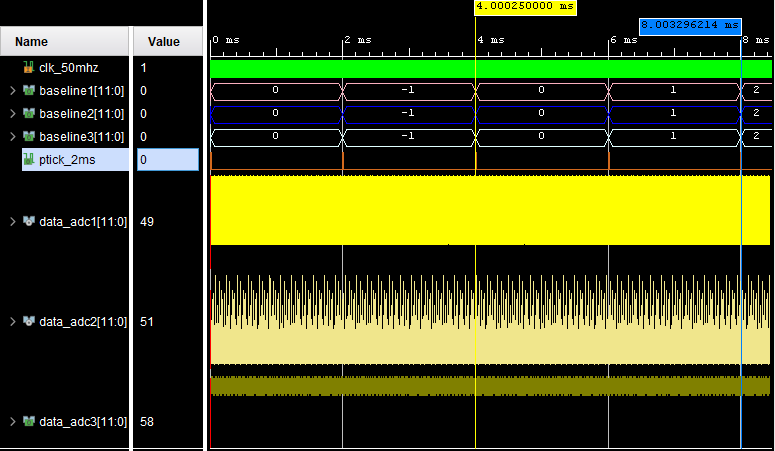
\includegraphics[width=0.9\textwidth]{Figs/actualbase.PNG} 
\centering
\caption{Simulación del comportamiento de las señales en baseline, versión actualizada}
\label{sim2ms}
\end{figure}

\subsection{Simulación Baseline versión (original y actualizada)}
En la simulación mostrada en la Figura~\ref{sim2ms} en color café se muestra la actualización de la señal (ptick\_2ms) con un período de 2ms.

A cada canal de entrada (data\_adc1, data\_adc2, data\_adc3) se le ingresa una señal diferente desde la memoria del hardwware externo. Las señales de salida (baseline\_1, baseline\_2, baseline\_3), tienen el mismo comportamiento, ya que en el diseño se tiene un contador que acumula por 2 ms los datos provenientes de cada canal y calcula un promedio del error en la entrada con respecto a una referencia de 50 mV que en este caso corresponde a 50 niveles de cuantización. La salida de este circuito será conectada a un DAC para generar el voltaje necesario y así, corregir el offset de línea base para mantener el sistema en estado estable.  

%Así, se logra la estabilización de la linea base por los niveles de cuantización entregados al DAC.


\begin{figure}[H]
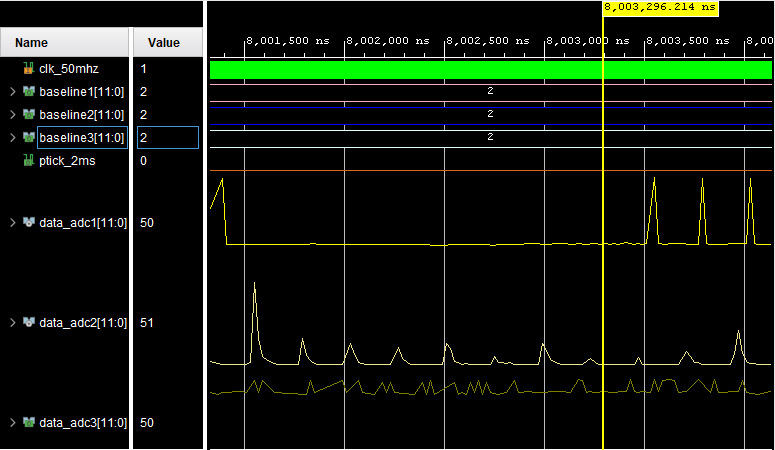
\includegraphics[width=0.9\textwidth]{Figs/zombasenue.PNG} 
\centering
\caption{Simulación de las entradas de baseline, versión actualizada}
\label{finbase}
\end{figure}

En la  Figura~\ref{finbase} se hace un acercamiento al cursor posicionado en 8,00329996214~ ms mostrado en la figura anterior, para observar el comportamiento de las entradas en forma análogica, nótese el  comportamiento diferente que tienen las tres entradas.

%\begin{itemize}
%    \item {\textbf{Simulación Baseline versión original}}
%\end{itemize}


El comportamiento en las señales de salida (baseline1, baseline2, baseline3) es similar logrando una actualización cada 2 ms.

%En la Figura~\ref{baseor}, el cursor amarillo se ubica en el mismo instante de tiempo que en Figura~\ref{finbase}, pero las entradas (data\_adc) no se encuentran en el mismo valor numerico que se presenta en la columna (value), eso se debe a la mejora en la frecuencia de la versión actualizada, que se implementa a 50 MHz con respeto a la original implementada a 40 MHz . De acuerdo a lo anterior los datos que se observan son diferentes, 



%se presentan las mismas señales del control de linea base con el fin de verificar el comportamiento similar, nótese algunas diferencias como el periodo de muestreo es de 25ns ya que se tiene una frecuencia menor y por tanto los datos que se observan en los cursores son diferentes. Sin embargo, el comportamiento de las salidas(baseline1, baseline2, baseline3) es similar y al igual se logra una actualización cada 2ms.
 
\begin{figure}[H]
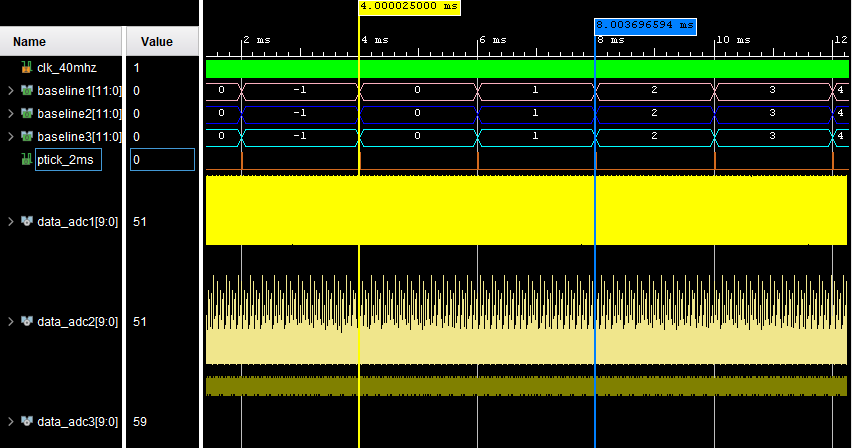
\includegraphics[width=0.9\textwidth]{Figs/baselineori.PNG} 
\centering
\caption{Simulación del comportamiento de las señales en baseline, versión original}
\label{actu4ms}
\end{figure}

En la Figura~\ref{baseor}, el cursor amarillo se ubica en el mismo instante de tiempo que en Figura~\ref{finbase}, pero las entradas (data\_adc) no se encuentran en el mismo valor numerico que se presenta en la columna (value), eso se debe a la mejora en la frecuencia de la versión actualizada, que se implementa a 50 MHz con respeto a la original implementada a 40 MHz . De acuerdo a lo anterior los datos que se observan son diferentes.

\begin{figure}[H]
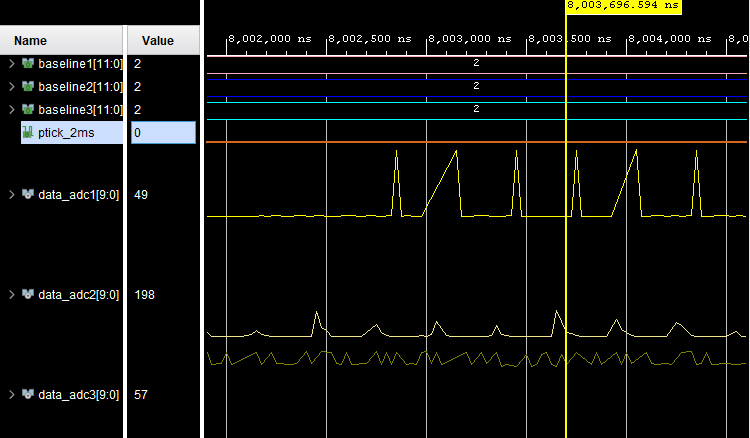
\includegraphics[width=0.9\textwidth]{Figs/zombase.PNG} 
\centering
\caption{Simulación de las entradas de baseline, versión original}
\label{baseor}
\end{figure}
%__________________________________________________________________________Seguir revisando 

\subsection{Simulación Rampa (original y actualizada)}
En esta simulación se evidencian algunos cambios realizados respecto al diseño original LAGO con el fin de aplicar unas mejoras. Una es la restricción del máximo valor que el usuario puede ingresar como parámetro de entrada DATA\_IN(1023) a la rampa.
Dado que en la versión original aunque el valor máximo efectivo es 1023, es posible ingresar un número mayor así no tenga efecto alguno en la generación de la señal de salida.

En la Figura~\ref{10ns} se puede observar las rampas que se generan a partir de tres valores de polarización que se ingresan en distintos instantes de tiempo por el usuario, con tiempo de 200 ms en estado estable para cada uno.

\begin{figure}[H]
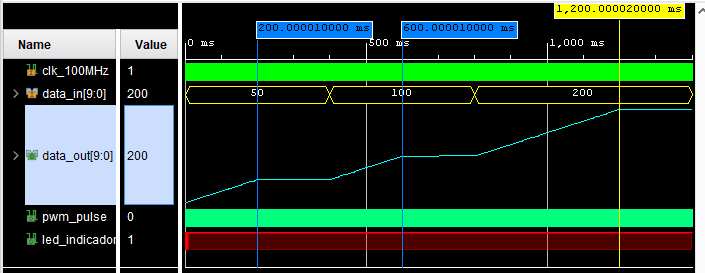
\includegraphics[width=0.9\textwidth]{Figs/Rampa_100Mhz.PNG} 
\centering
\caption{Simulación rampa de polarización del proyecto LAGO, versión actualizada}
\label{10ns}
\end{figure}
En Figura~\ref{10ns2} se observa un acercamiento donde se puede apreciar el comportamiento del ciclo útil en la señal (PWM\_pulse) con duración de 20 ns.


\begin{figure}[H]
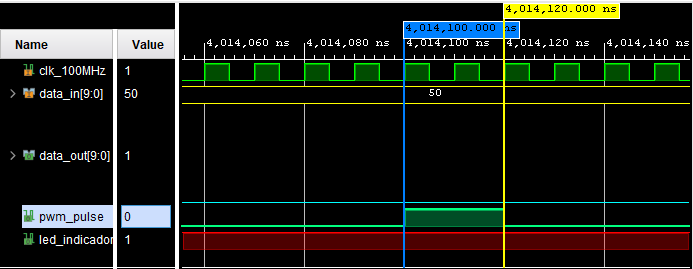
\includegraphics[width=0.9\textwidth]{Figs/zomnuevo.PNG} \centering
\caption{Ciclo útil de 10 ns para la PWM del proyecto LAGO, versión actualizada}
\label{10ns2}
\end{figure}


\begin{itemize}
    \item {\textbf{Simulación Rampa versión original}}
\end{itemize}

Para estimular este diseño se ingresa un \texttt{DATA\_IN} de 1023, de igual manera se estimula con un período de 20~ns ya que la frecuencia de la FPGA utilizada es de 50 MHz.
La salida (data\_out) cambia cada 4 ms como se muestra en la Figura~\ref{ciclo10}.

\begin{figure}[H]
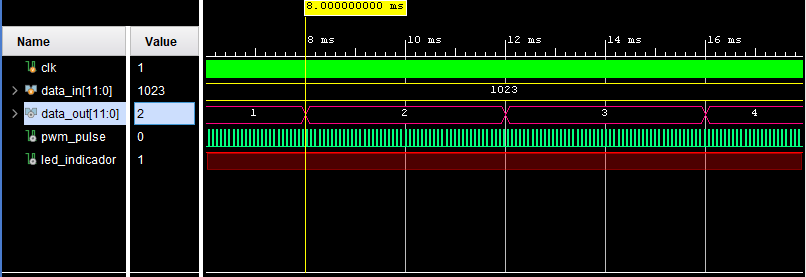
\includegraphics[width=0.9\textwidth]{Figs/pwmoriginal.PNG} 
\centering
\caption{Actualización de la PWM del proyecto LAGO, versión original}
\label{actualizacionac}
\end{figure}

A diferencia del diseño original de LAGO este diseño tiene un ciclo útil de 20 ns lo cual se evidencia en logrando actualizar la PWM de manera más rápida.

\begin{figure}[H]
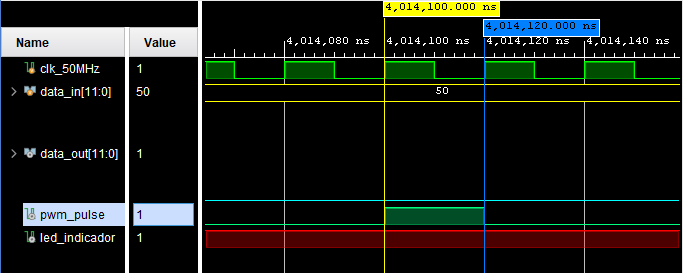
\includegraphics[width=0.9\textwidth]{Figs/zomviejo.PNG} 
\centering
\caption{Ciclo útil de 20ns para la PWM del proyecto LAGO, versión original}
\label{ciclo10}
\end{figure}

\begin{figure}[H]
 \centering
 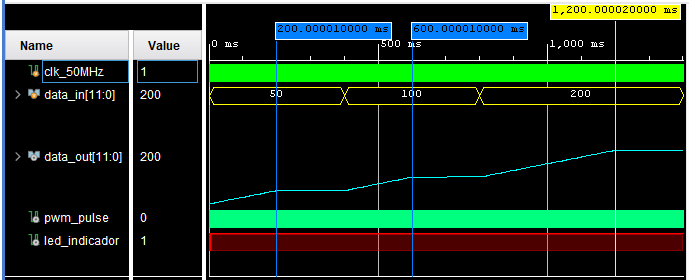
\includegraphics[width=0.9\textwidth]{Figs/Rampa_50MHz.PNG}
 \caption{Ciclo útil de 20ns para la PWM del proyecto LAGO, versión original}
 \label{ramapa50}
\end{figure}

En la Figura~\ref{ramapa50} se estimula el circuito con las condiciones presentadas en la Figura~\ref{10ns}.

Las simulaciones evidencian que las dos versiones presentan el mismo tiempo de establecimiento el cual se puede ver en los cursores de la Figura~\ref{ramapa50} y la Figura~\ref{10ns}. De lo anterior podemos concluir que conserva la misma respuesta la señal de salida.



\subsection{Simulación Trigger (original y actual)}
Las señales se estimulan con un reloj de periodo 20 ns.
%Se estimulan las señales con un periodo de 20ns, en la Figura~\ref{tigeer} El segmento extraido expone el funcionamento del circuito para la discriminación de datos llamado Trigger.

\begin{figure}[H]
\centering
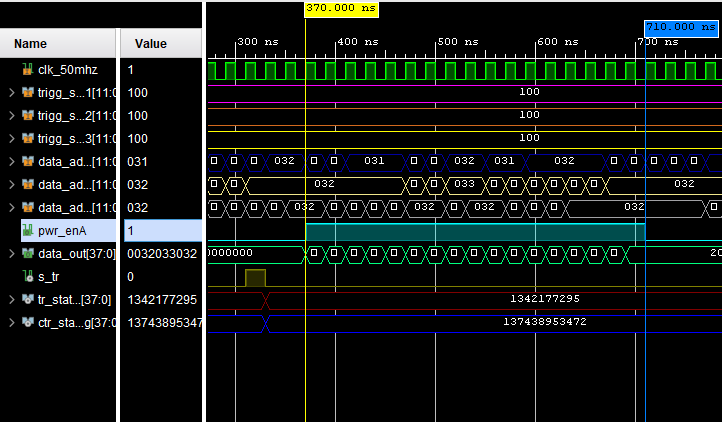
\includegraphics[width=0.9\textwidth]{Figs/trigernevo.PNG} 
\caption{Señales de Trigger destacadas del proyecto LAGO, versión actualizada}
\label{tigeer}
\end{figure}

La simulación muestra el circuto en estado de detección que evidencia la secuencia de señales necesarias para el almacenamiento del evento considerado rayo cósmico. Ver Figura~\ref{tigeer}

La señal (s\_tr) se activa en el momento que cualquier canal de entrada (Data\_adc) supera sus respectivos umbrales (trigger\_set), dos ciclos de reloj después, se pone en alto (pwr\_enA) durante 340 ns indicando que se almacenarán las 15 muestras que ingresan de la captura.\\
La señal (data\_out) concatena las muestras de los tres canales para su posterior comunicación por protocolo SPI con la Raspberry Pi, de modo que se envían consecutivamente 15 tramas de datos correspondientes al evento y dos adicionales para los contadores (tr\_status\_reg) y (ctr\_status\_reg).


%, pwr\_enA se pone en alto cuando se tiene información para almacenar, a su vez se evidencia data\_out una señal de 38 bits entrega la información del evento en 340ns; 15 ciclos de muestras seguidos por 2 ciclos más que entregan los contadores(tr\_status\_reg) y (ctr\_status\_reg).
%Nótese además en esta figura la posibilidad de disparo(s\_tr) en cualquiera de los 3 canales ya que se establece el mismo umbral de activación en (trigger1, trigger2, trigger3),



%cabe resaltar el ingreso de valores diferentes en las  entradas(data\_adc1,data\_adc2,data\_adc3) y el cursor posicionado en 370ns para evidenciar la bandera de 2 bits y el registro de las muestras en los 3 canales en orden ascendente.

\begin{itemize}
    \item {\textbf{Simulación Trigger versión original}}
    
\end{itemize}

En  la Figura~\ref{trigerlago} cabe notar algunas diferencias que se presentan por las mejoras realizadas al diseño. Se estimularon las señales con un reloj de 40 MHz, Data\_out se respresenta en 32 bits, el tiempo en que pwr\_enA esta en alto de 350 ns. Al igual que la figura anterior se establecen los mismo estímulos de entrada para evidenciar un comportamiento similar en los diseños.
\begin{figure}[H]
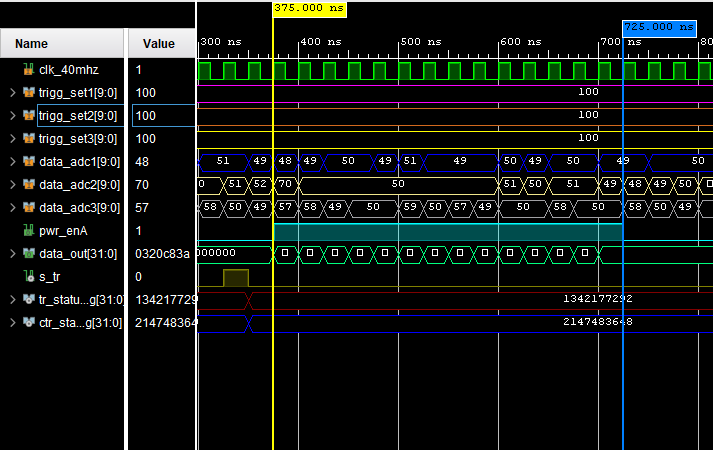
\includegraphics[width=0.9\textwidth]{Figs/trigerviejo.PNG} 
\centering
\caption{Señales de Trigger destacadas del proyecto LAGO, versión original}
\label{trigerlago}
\end{figure}

Como se evidencia en cada una de las simulaciones se logra obtener un resultado equivalente en las señales de control que componen el procesamiento de datos del proyecto LAGO y algunas mejoras como el aumento en la frecuencia de muestreo.

\section{\textbf{Salida de control para PMT's}}
A continuación se muestran graficas de la señal PWM obtenida luego de implementar en FPGA los diseños expuestos en Capítulo 3.

\begin{figure}[H]
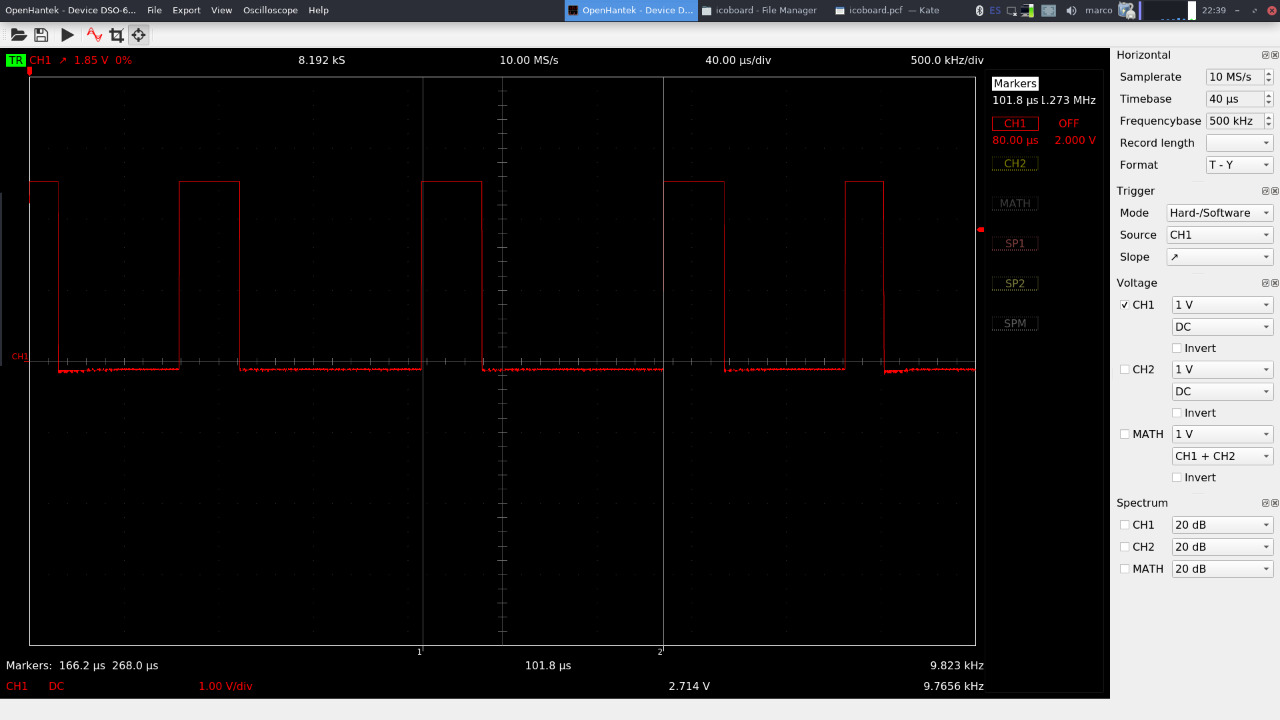
\includegraphics[width=0.9\textwidth]{Figs/PWM 2.jpeg} 
\centering
\caption{Señal de control PWM, versión actualizada}
\label{pwmactual}
\end{figure}
\begin{figure}[H]

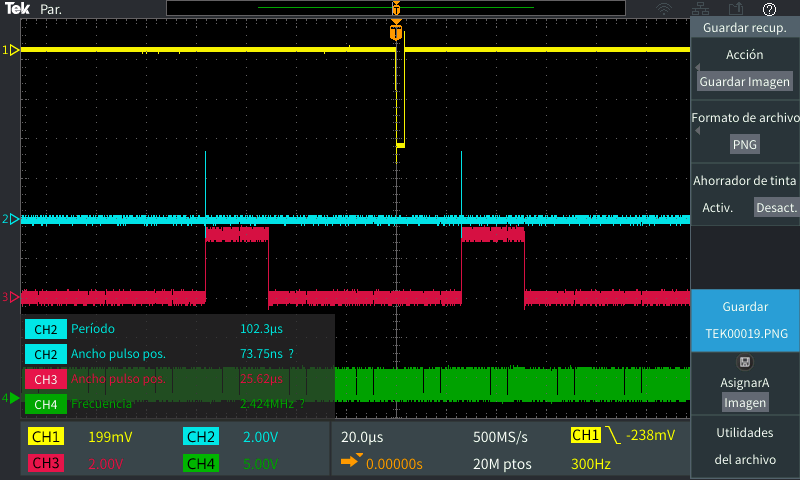
\includegraphics[width=0.9\textwidth]{Figs/TEK00019.PNG} 
\centering
\caption{Señal de control PWM, versión actual}
\label{pwmantigua}
\end{figure}


En la Figura ~\ref{pwmactual} se obtiene una señal que cumple con una frecuencia medida en osciloscopio de 9,823 KHz de ciclo útil variable y un voltaje máximo de 2,714 V.

En la Figura~\ref{pwmantigua} se observa la señal PWM en el CH2 con un período de 102,3 us equivalente a una frecuencia de 9,775 KHz con un ciclo útil varible.


\section{\textbf{Registro de datos}}
En primer lugar se resalta la terminal de usuario Figura~\ref{adecuacion} en la que se ingresan cada uno de los umbrales ya explicados durante el desarrollo del proyecto.

%En esta terminal se hacen algunas abreviaturas de las constantes que pueden aparecer duante el registro y el almacenamiento de la información.

\begin{figure}[H]
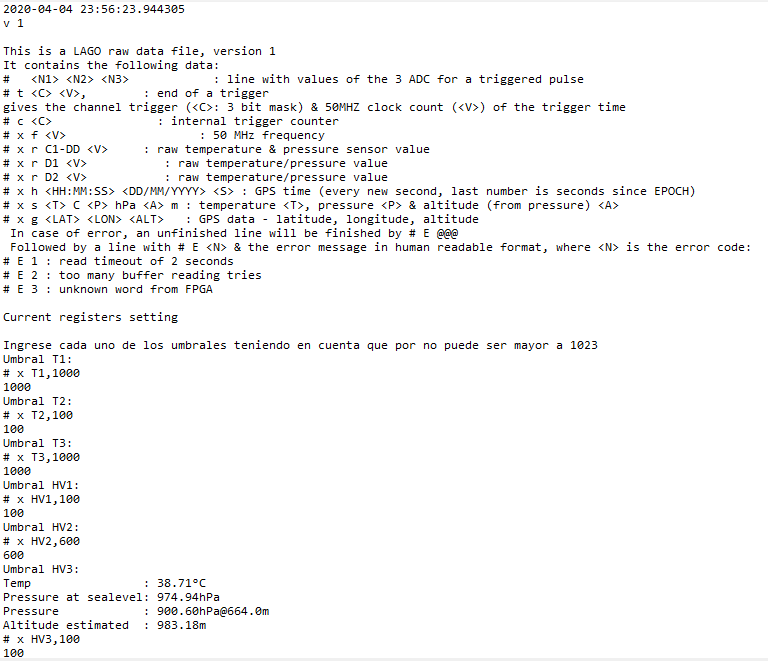
\includegraphics[width=0.95\textwidth]{Figs/terminal.PNG} 
\centering
\caption{Cabecera del archivo de datos del terminal de usuario proyecto LAGO}
\label{adecuacion}
\end{figure}

Luego de la implementación se obtiene el siguiente archivo de salida en el cual se evidencia la correcta comunicación entre la Icoboard y la Raspberry Pi para registrar el evento proveniente de la FPGA Nexys 4 a una frecuencia de 50 MHz. 

En la Figura~\ref{mta} se muestra en recuadro rojo un recorte de uno de los eventos obtenidos en el archivo de salida como resultado de este proyecto, y en recuadro azul un recorte de uno de los eventos tomado como referencia del proyecto LAGO. 

\begin{figure}[H]
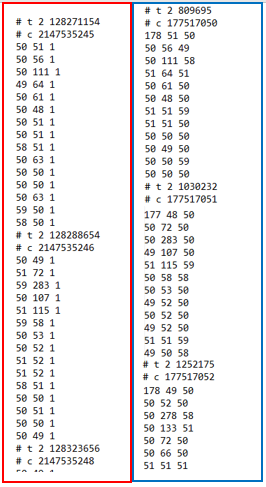
\includegraphics[scale=0.9]{Figs/eventos.PNG} 
\centering
\caption[Comparación de archivos de salida con datos de eventos considerados rayos cósmicos]{Comparación de archivos de salida con datos de eventos considerados rayos cósmicos. *\textbf{Cuadro rojo:} versión actualizada. *\textbf{Cuadro azul:}versión original}
\label{mta}
\end{figure}


En la Figura~\ref{adecuacion} se muestra un evento para corrobar el funcionamiento del diseño implementado y mostrar el comportamiento de los datos obtenidos, además, una interpolación de las muestras registradas usando Matlab~\textregistered~ para tener un acercamiento real de la forma del pulso de un evento considerado rayo cósmico.

\begin{figure}[H]
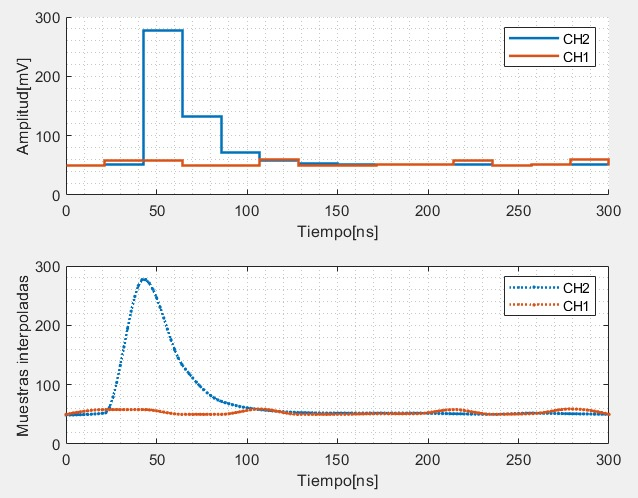
\includegraphics[width=0.9\textwidth]{Figs/salidadata.jpeg} 
\centering
\caption[Gráfica de evento hardware vs pulso interpolado]{(Arriba) Gráfica discreta de un evento registrado por el hardware diseñado.(Abajo) pulso interpolado}
\label{adecuacion}
\end{figure}

En las siguientes gráficas se resume el comportamiento de los datos entregados por el sensor de presión y temperatura.

\begin{figure}[H]
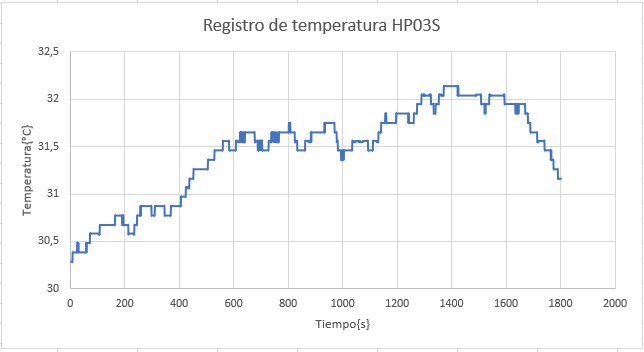
\includegraphics[width=0.9\textwidth]{Figs/TEMPERATURA.PNG} 
\centering
\caption{Registro de temperatura HP03S durante un registro de media hora}
\label{temp}
\end{figure}

\begin{figure}[H]
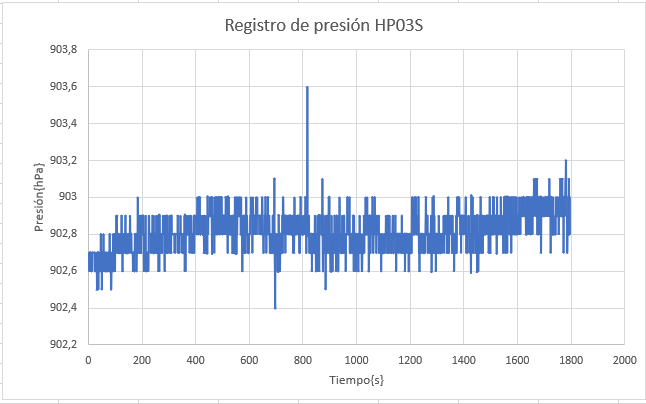
\includegraphics[width=0.9\textwidth]{Figs/presion.PNG} 
\centering
\caption{Registro de presión HP03S durante un tiempo de registro de media hora}
\label{pre}
\end{figure}


% ------------------------------------------------------------------------ 